\documentclass[a4paper,12pt]{article}
\usepackage[top = 2.5cm, bottom = 2.5cm, left = 2.5cm, right = 2.5cm]{geometry}
\usepackage[T1]{fontenc}
\usepackage[utf8]{inputenc}
\usepackage{multirow} 
\usepackage{booktabs} 
\usepackage{graphicx}
\usepackage[spanish]{babel}
\usepackage{setspace}
\setlength{\parindent}{0in}
\usepackage{float}
\usepackage{fancyhdr}
\usepackage{amsmath}
\usepackage{amssymb}
\usepackage{amsthm}
\usepackage[numbers]{natbib}
\newcommand\Mycite[1]{%
	\citeauthor{#1}~[\citeyear{#1}]}
\usepackage{graphicx}
\usepackage{subcaption}
\usepackage{booktabs}
\usepackage{etoolbox}
\usepackage{minibox}
\usepackage{hyperref}
\usepackage{xcolor}
\usepackage[skins]{tcolorbox}
%---------------------------

\newtcolorbox{cajita}[1][]{
	 #1
}

\newenvironment{sol}
{\renewcommand\qedsymbol{$\square$}\begin{proof}[\textbf{Solución.}]}
	{\end{proof}}

\newenvironment{dem}
{\renewcommand\qedsymbol{$\blacksquare$}\begin{proof}[\textbf{Demostración.}]}
	{\end{proof}}

\newtheorem{problema}{Problema}
\newtheorem{definicion}{Definición}
\newtheorem{ejemplo}{Ejemplo}
\newtheorem{teorema}{Teorema}
\newtheorem{corolario}{Corolario}[teorema]
\newtheorem{lema}[teorema]{Lema}
\newtheorem{prop}{Proposición}
\newtheorem*{nota}{\textbf{NOTA}}
\renewcommand\qedsymbol{$\blacksquare$}
\usepackage{svg}
\usepackage{tikz}
\usepackage[framemethod=default]{mdframed}
\global\mdfdefinestyle{exampledefault}{%
linecolor=lightgray,linewidth=1pt,%
leftmargin=1cm,rightmargin=1cm,
}




\newenvironment{noter}[1]{%
\mdfsetup{%
frametitle={\tikz\node[fill=white,rectangle,inner sep=0pt,outer sep=0pt]{#1};},
frametitleaboveskip=-0.5\ht\strutbox,
frametitlealignment=\raggedright
}%
\begin{mdframed}[style=exampledefault]
}{\end{mdframed}}
\newcommand{\linea}{\noindent\rule{\textwidth}{3pt}}
\newcommand{\linita}{\noindent\rule{\textwidth}{1pt}}

\AtBeginEnvironment{align}{\setcounter{equation}{0}}
\pagestyle{fancy}

\fancyhf{}









%----------------------------------------------------------
\lhead{\footnotesize Modelación y Simulación}
\rhead{\footnotesize  Rudik Roberto Rompich}
\cfoot{\footnotesize \thepage}


%--------------------------

\begin{document}
 \thispagestyle{empty} 
    \begin{tabular}{p{15.5cm}}
    \begin{tabbing}
    \textbf{Universidad del Valle de Guatemala} \\
    Departamento de Matemática\\
    Licenciatura en Matemática Aplicada\\\\
   \textbf{Estudiante:} Rudik Roberto Rompich\\
   \textbf{Correo:}  \href{mailto:rom19857@uvg.edu.gt}{rom19857@uvg.edu.gt}\\
   \textbf{Carné:} 19857
    \end{tabbing}
    \begin{center}
        CC3039 - Modelación y Simulación - Catedrático: Oseas Paredes\\
        \today
    \end{center}\\
    \hline
    \\
    \end{tabular} 
    \vspace*{0.3cm} 
    \begin{center} 
    {\Large \bf Microproyecto 1
} 
        \vspace{2mm}
    \end{center}
    \vspace{0.4cm}
%--------------------------

El siguiente proyecto tiene como objeto completar las ideas desarrolladas en clase. Su trabajo consistirá en presentar lo que se le indica en formato PDF (no tome fotos), debidamente escaneadas. NO OLVIDE ESCRIBIR SU NOMBRE Y NÚMERO DE CARNÉ. 

\begin{enumerate}
	\item ¿Cuáles son los métodos sistemáticos que se usan en ciencia a fin de encontrar las leyes que gobiernan el universo observable?
	\begin{sol}
		Son tres métodos: 
		\begin{enumerate}
			\item Método deductivo (axiomático).
			\item Método inductivo (científico).
		\end{enumerate}
	\end{sol}
	
	\item Defina en sus propias palabras cada uno de los métodos usados en ciencia.
	\begin{sol}
		Tenemos: 
		\begin{enumerate}
			\item \textbf{Método deductivo (axiomático)}. Es la forma en que las matemáticas se escriben, es decir, como los axiomas de Zermelo-Fraenkel de la teoría de conjuntos; en donde a partir de ellos, todas las matemáticas se deducen. Este método parte de lo más elemental y se dirige hacia lo más particular o complejo. 
			\item \textbf{Método inductivo (científico)}. Su característica principal es el uso del método científico, es decir, a partir de experimentos se determinan propiedades que gobiernan el cosmos. 
		\end{enumerate}
	\end{sol}

	\item ¿Cuál es el nombre de la disciplina que sistematiza los primeros tres pasos del método científico (inductivo)?
	\begin{sol}
		La estadística.
	\end{sol}
	
	\item ¿Escriba los términos usuales en la nomenclatura del Método Deductivo?
	\begin{sol} Se tienen:
	\begin{enumerate}
		\item Definición.
		\item Términos primitivos. 
		\item Demostración.
		\item Axioma.
		\item Postulado. 
		\item Teorema. 
		\item Corolario.
		\item Converso.
		\item Lema.
		\item Escolio.
	\end{enumerate}
\end{sol}
	
	\item ¿Cuáles son las limitantes del método deductivo?
	\begin{sol}
		Por el Teorema de Incompletud de Gödel, toda teoría consistente es incompleta. Es decir, el método deductivo no puede deducir todas las verdades matemáticas. 
	\end{sol}
	
	\item ¿Cuáles son las limitantes del método inductivo (científico)?
	\begin{sol}
		El principal problema es que la ciencia otorga condiciones suficientes; pero no las necesarias en la mayoría de casos. Algunos ejemplos interesantes: principio de incertidumbre de Heisenberg y el teorema del límite central. 
	\end{sol}
	
	\item Explique en sus propias palabras de qué trata el Teorema de Incompletud de Gödel.
	
	\begin{sol}
		En palabras sencillas, lo que nos dice el teorema es que en cualquier sistema formal inductivo siempre habrán cuestiones que no puedan ser demostradas o que este libre de contradicciones.
	\end{sol}
	\item Explique en sus propias palabras de qué trata el Principio de Incertidumbre de Heisenberg.
	\begin{sol}
		Lo que nos dice es que la incertidumbre es adherente a cualquier partícula, por lo general se le asocia a la posición y al momento de la partícula. Es decir, mientras se conozca el momento entonces la posición es más incerta; y viceversa. 
	\end{sol}
	
	\item Describa en sus propias palabras qué dice el Teorema del Límite Central de Gauss y dé una interpretación filosófica que afecte al método científico.
	\begin{sol}
		El teorema en cuestión, nos dice que si tenemos un experimento con muestras obtenidas de varias observaciones generadas aleatoriamente entonces la distribución de probabilidad tenderá a una distribución normal. El problema que surge con el método científico, es que es prácticamente imposible generar observaciones infinitas. 
	\end{sol}
	
	\item Describa la relación filosófica entre el Teorema del Límite Central y el Principio de Incertidumbre de Heisenberg. 
	\begin{sol}
		El problema filosófico surge debido a que los humanos no estamos acostumbrados a esperar resultados inciertos en el macrouniverso; usualmente las cuestiones se resuelven con un sí o un no. Sin embargo, en el caso de estas dos cuestiones, los resultados no son intuitivamente satisfactorias, ya que la respuesta no es concisa. 
	\end{sol}
	\item La siguiente tabla contiene los pesos de 40 estudiantes en la universidad Princeton, que se registran con aproximación de una librería (este es un ejemplo de toma de datos).
	\begin{center}
		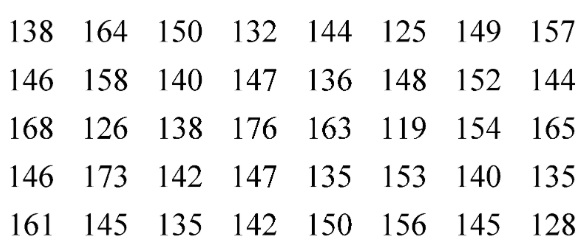
\includegraphics[scale=0.4]{images/1}
	\end{center}

	\begin{enumerate}
		\item Ordene los datos de menor a mayor y establezca el rango ($\varrho$) de los datos.
		\item Construya una tabla de distribución de frecuencias y asigne probabilidades (discretas) a cada intervalo asociado (Ayuda: Una elección conveniente para el tamaño del intervalo de clase es de 5lb.)
		\item Establezca las marcas de clase para cada uno de los intervalos de clase de la tabla de distribución de frecuencias anterior.
		\item En la misma tabla construya los intervalos con límites reales para las clases originales, conservando el tamaño y las marcas de clase de las mismas.
		\item Construya un histograma y un polígono de frecuencias asociada a la tabla de distribución de frecuencias.
	\end{enumerate}
\end{enumerate}

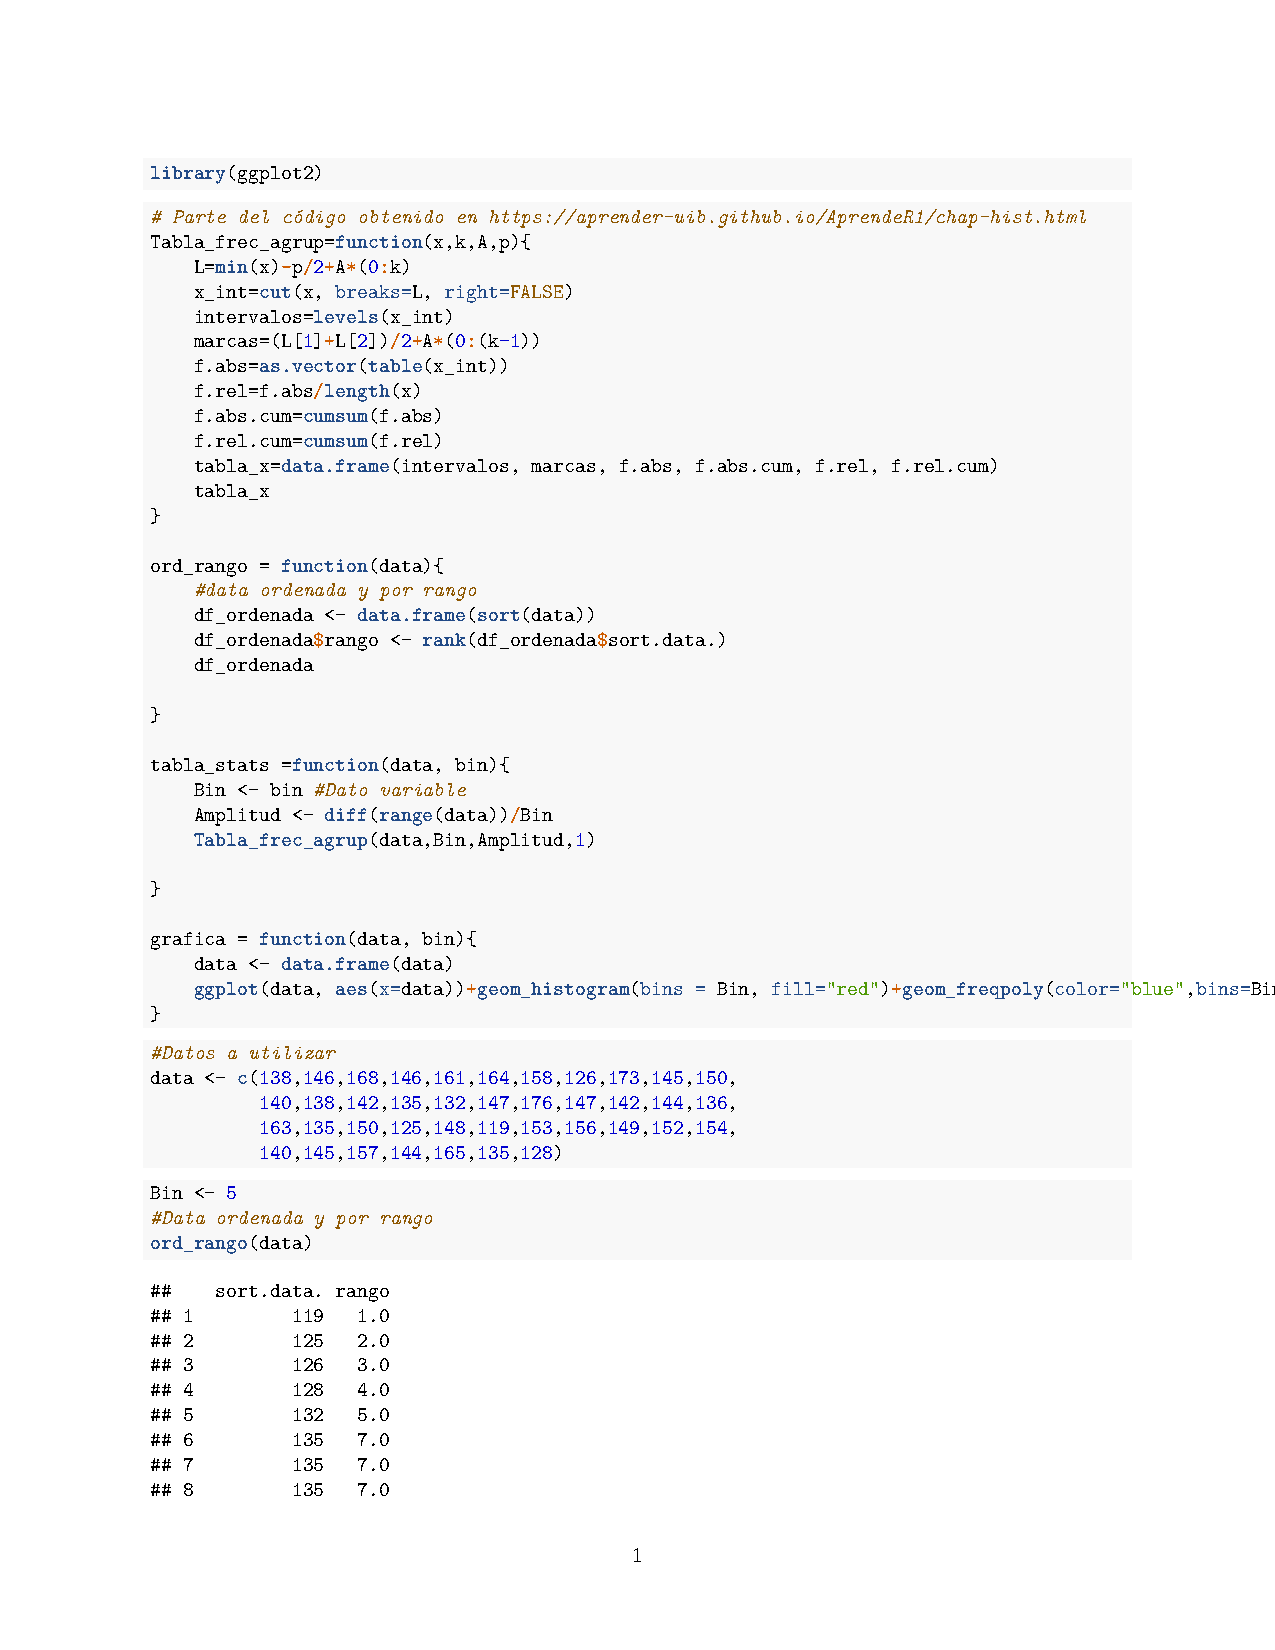
\includepdf[pages=-]{images/problema-10.pdf}



%---------------------------
%\bibliographystyle{apa}
%\bibliography{referencias.bib}

\end{document}